\documentclass[twoside]{book}

% Packages required by doxygen
\usepackage{fixltx2e}
\usepackage{calc}
\usepackage{doxygen}
\usepackage[export]{adjustbox} % also loads graphicx
\usepackage{graphicx}
\usepackage[utf8]{inputenc}
\usepackage{makeidx}
\usepackage{multicol}
\usepackage{multirow}
\PassOptionsToPackage{warn}{textcomp}
\usepackage{textcomp}
\usepackage[nointegrals]{wasysym}
\usepackage[table]{xcolor}

% Font selection
\usepackage[T1]{fontenc}
\usepackage[scaled=.90]{helvet}
\usepackage{courier}
\usepackage{amssymb}
\usepackage{sectsty}
\renewcommand{\familydefault}{\sfdefault}
\allsectionsfont{%
  \fontseries{bc}\selectfont%
  \color{darkgray}%
}
\renewcommand{\DoxyLabelFont}{%
  \fontseries{bc}\selectfont%
  \color{darkgray}%
}
\newcommand{\+}{\discretionary{\mbox{\scriptsize$\hookleftarrow$}}{}{}}

% Page & text layout
\usepackage{geometry}
\geometry{%
  a4paper,%
  top=2.5cm,%
  bottom=2.5cm,%
  left=2.5cm,%
  right=2.5cm%
}
\tolerance=750
\hfuzz=15pt
\hbadness=750
\setlength{\emergencystretch}{15pt}
\setlength{\parindent}{0cm}
\setlength{\parskip}{3ex plus 2ex minus 2ex}
\makeatletter
\renewcommand{\paragraph}{%
  \@startsection{paragraph}{4}{0ex}{-1.0ex}{1.0ex}{%
    \normalfont\normalsize\bfseries\SS@parafont%
  }%
}
\renewcommand{\subparagraph}{%
  \@startsection{subparagraph}{5}{0ex}{-1.0ex}{1.0ex}{%
    \normalfont\normalsize\bfseries\SS@subparafont%
  }%
}
\makeatother

% Headers & footers
\usepackage{fancyhdr}
\pagestyle{fancyplain}
\fancyhead[LE]{\fancyplain{}{\bfseries\thepage}}
\fancyhead[CE]{\fancyplain{}{}}
\fancyhead[RE]{\fancyplain{}{\bfseries\leftmark}}
\fancyhead[LO]{\fancyplain{}{\bfseries\rightmark}}
\fancyhead[CO]{\fancyplain{}{}}
\fancyhead[RO]{\fancyplain{}{\bfseries\thepage}}
\fancyfoot[LE]{\fancyplain{}{}}
\fancyfoot[CE]{\fancyplain{}{}}
\fancyfoot[RE]{\fancyplain{}{\bfseries\scriptsize Generated by Doxygen }}
\fancyfoot[LO]{\fancyplain{}{\bfseries\scriptsize Generated by Doxygen }}
\fancyfoot[CO]{\fancyplain{}{}}
\fancyfoot[RO]{\fancyplain{}{}}
\renewcommand{\footrulewidth}{0.4pt}
\renewcommand{\chaptermark}[1]{%
  \markboth{#1}{}%
}
\renewcommand{\sectionmark}[1]{%
  \markright{\thesection\ #1}%
}

% Indices & bibliography
\usepackage{natbib}
\usepackage[titles]{tocloft}
\setcounter{tocdepth}{3}
\setcounter{secnumdepth}{5}
\makeindex

% Hyperlinks (required, but should be loaded last)
\usepackage{ifpdf}
\ifpdf
  \usepackage[pdftex,pagebackref=true]{hyperref}
\else
  \usepackage[ps2pdf,pagebackref=true]{hyperref}
\fi
\hypersetup{%
  colorlinks=true,%
  linkcolor=blue,%
  citecolor=blue,%
  unicode%
}

% Custom commands
\newcommand{\clearemptydoublepage}{%
  \newpage{\pagestyle{empty}\cleardoublepage}%
}

\usepackage{caption}
\captionsetup{labelsep=space,justification=centering,font={bf},singlelinecheck=off,skip=4pt,position=top}

%===== C O N T E N T S =====

\begin{document}

% Titlepage & ToC
\hypersetup{pageanchor=false,
             bookmarksnumbered=true,
             pdfencoding=unicode
            }
\pagenumbering{roman}
\begin{titlepage}
\vspace*{7cm}
\begin{center}%
{\Large Hello }\\
\vspace*{1cm}
{\large Generated by Doxygen 1.8.11}\\
\end{center}
\end{titlepage}
\clearemptydoublepage
\tableofcontents
\clearemptydoublepage
\pagenumbering{arabic}
\hypersetup{pageanchor=true}

%--- Begin generated contents ---
\chapter{File Index}
\section{File List}
Here is a list of all files with brief descriptions\+:\begin{DoxyCompactList}
\item\contentsline{section}{src/\hyperlink{hello_8c}{hello.\+c} }{\pageref{hello_8c}}{}
\item\contentsline{section}{src/\hyperlink{system_8h}{system.\+h} }{\pageref{system_8h}}{}
\end{DoxyCompactList}

\chapter{File Documentation}
\hypertarget{hello_8c}{}\section{src/hello.c File Reference}
\label{hello_8c}\index{src/hello.\+c@{src/hello.\+c}}
{\ttfamily \#include $<$config.\+h$>$}\\*
{\ttfamily \#include $<$getopt.\+h$>$}\\*
{\ttfamily \#include $<$stdnoreturn.\+h$>$}\\*
{\ttfamily \#include $<$wchar.\+h$>$}\\*
{\ttfamily \#include \char`\"{}system.\+h\char`\"{}}\\*
{\ttfamily \#include \char`\"{}closeout.\+h\char`\"{}}\\*
{\ttfamily \#include \char`\"{}configmake.\+h\char`\"{}}\\*
{\ttfamily \#include \char`\"{}dirname.\+h\char`\"{}}\\*
{\ttfamily \#include \char`\"{}errno.\+h\char`\"{}}\\*
{\ttfamily \#include \char`\"{}error.\+h\char`\"{}}\\*
{\ttfamily \#include \char`\"{}gettext.\+h\char`\"{}}\\*
{\ttfamily \#include \char`\"{}progname.\+h\char`\"{}}\\*
{\ttfamily \#include \char`\"{}xalloc.\+h\char`\"{}}\\*
{\ttfamily \#include \char`\"{}ctype.\+h\char`\"{}}\\*
{\ttfamily \#include $<$stdio.\+h$>$}\\*
{\ttfamily \#include $<$gtk/gtk.\+h$>$}\\*
{\ttfamily \#include $<$gdk/gdk.\+h$>$}\\*
Include dependency graph for hello.\+c\+:\nopagebreak
\begin{figure}[H]
\begin{center}
\leavevmode
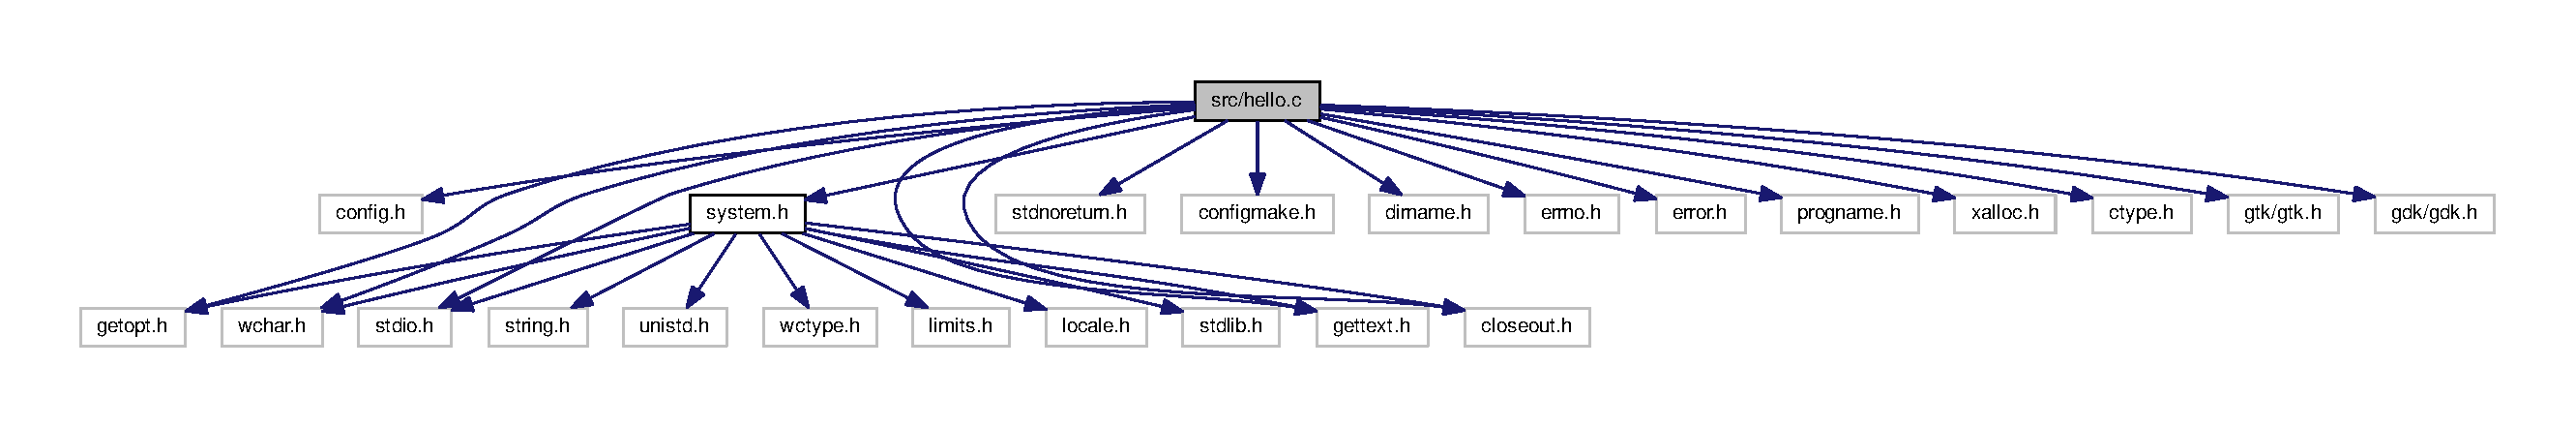
\includegraphics[width=350pt]{hello_8c__incl}
\end{center}
\end{figure}
\subsection*{Functions}
\begin{DoxyCompactItemize}
\item 
static \+\_\+\+Noreturn void \hyperlink{hello_8c_a6fc4beeab8ac72edc27edc24cf7ef525}{print\+\_\+help} (F\+I\+LE $\ast$restrict out)
\item 
static void \hyperlink{hello_8c_a2e0d36c06cdd7fbacb264c67367d3b01}{print\+\_\+version} (void)
\item 
static void \hyperlink{hello_8c_a9327e4e5f8a3d809ecf0e564973b091b}{print\+\_\+simbols} (const char $\ast$)
\item 
static void \hyperlink{hello_8c_a16ede0b83ba9386247c53f9ef3650321}{gtk\+\_\+greeting} (const char $\ast$greeting\+\_\+msg)
\item 
int \hyperlink{hello_8c_a0ddf1224851353fc92bfbff6f499fa97}{main} (int argc, char $\ast$argv\mbox{[}$\,$\mbox{]})
\end{DoxyCompactItemize}
\subsection*{Variables}
\begin{DoxyCompactItemize}
\item 
static const struct option \hyperlink{hello_8c_a7f2c8becae59a68faf6fc1540e88ab11}{longopts} \mbox{[}$\,$\mbox{]}
\end{DoxyCompactItemize}


\subsection{Function Documentation}
\index{hello.\+c@{hello.\+c}!gtk\+\_\+greeting@{gtk\+\_\+greeting}}
\index{gtk\+\_\+greeting@{gtk\+\_\+greeting}!hello.\+c@{hello.\+c}}
\subsubsection[{\texorpdfstring{gtk\+\_\+greeting(const char $\ast$greeting\+\_\+msg)}{gtk_greeting(const char *greeting_msg)}}]{\setlength{\rightskip}{0pt plus 5cm}static void gtk\+\_\+greeting (
\begin{DoxyParamCaption}
\item[{const char $\ast$}]{greeting\+\_\+msg}
\end{DoxyParamCaption}
)\hspace{0.3cm}{\ttfamily [static]}}\hypertarget{hello_8c_a16ede0b83ba9386247c53f9ef3650321}{}\label{hello_8c_a16ede0b83ba9386247c53f9ef3650321}
Используя G\+TK выводит сообение в отдельном окне Здесь предполагается, что gtk\+\_\+parse\+\_\+args уже была вызвана ранее.

T\+O\+DO\+: проверить, удалось ли открыть дисплей.

G\+T\+K+ использует U\+T\+F-\/8, а строка greeting\+\_\+msg в системной кодировке, которая может отличаться.

T\+O\+DO\+: проверить, удалось ли преобразовать строку. 

Here is the caller graph for this function\+:\nopagebreak
\begin{figure}[H]
\begin{center}
\leavevmode
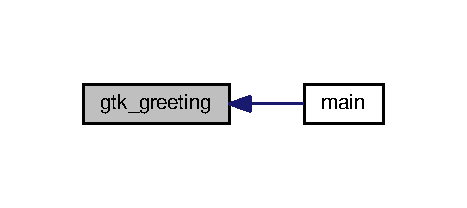
\includegraphics[width=224pt]{hello_8c_a16ede0b83ba9386247c53f9ef3650321_icgraph}
\end{center}
\end{figure}


\index{hello.\+c@{hello.\+c}!main@{main}}
\index{main@{main}!hello.\+c@{hello.\+c}}
\subsubsection[{\texorpdfstring{main(int argc, char $\ast$argv[])}{main(int argc, char *argv[])}}]{\setlength{\rightskip}{0pt plus 5cm}int main (
\begin{DoxyParamCaption}
\item[{int}]{argc, }
\item[{char $\ast$}]{argv\mbox{[}$\,$\mbox{]}}
\end{DoxyParamCaption}
)}\hypertarget{hello_8c_a0ddf1224851353fc92bfbff6f499fa97}{}\label{hello_8c_a0ddf1224851353fc92bfbff6f499fa97}
Set the text message domain.

Having initialized gettext, get the default message.

Even exiting has subtleties. On exit, if any writes failed, change the exit status. The /dev/full device on G\+N\+U/\+Linux can be used for testing; for instance, hello $>$/dev/full should exit unsuccessfully. This is implemented in the Gnulib module \char`\"{}closeout\char`\"{}.

--help and --version exit immediately, per G\+NU coding standards.

Print error message and exit. 

Here is the call graph for this function\+:\nopagebreak
\begin{figure}[H]
\begin{center}
\leavevmode
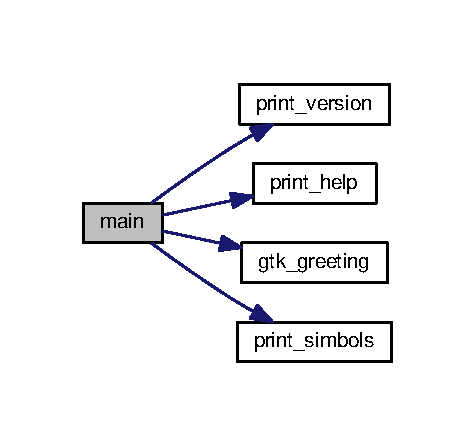
\includegraphics[width=228pt]{hello_8c_a0ddf1224851353fc92bfbff6f499fa97_cgraph}
\end{center}
\end{figure}


\index{hello.\+c@{hello.\+c}!print\+\_\+help@{print\+\_\+help}}
\index{print\+\_\+help@{print\+\_\+help}!hello.\+c@{hello.\+c}}
\subsubsection[{\texorpdfstring{print\+\_\+help(\+F\+I\+L\+E $\ast$restrict out)}{print_help(FILE *restrict out)}}]{\setlength{\rightskip}{0pt plus 5cm}static \+\_\+\+Noreturn void print\+\_\+help (
\begin{DoxyParamCaption}
\item[{F\+I\+LE $\ast$restrict}]{out}
\end{DoxyParamCaption}
)\hspace{0.3cm}{\ttfamily [static]}}\hypertarget{hello_8c_a6fc4beeab8ac72edc27edc24cf7ef525}{}\label{hello_8c_a6fc4beeab8ac72edc27edc24cf7ef525}
Справка по ключам

Print help info. This long message is split into several pieces to help translators be able to align different blocks and identify the various pieces. T\+R\+A\+N\+S\+L\+A\+T\+O\+RS\+: --help output 1 (synopsis) no-\/wrap

T\+R\+A\+N\+S\+L\+A\+T\+O\+RS\+: --help output 2 (brief description) no-\/wrap

T\+R\+A\+N\+S\+L\+A\+T\+O\+RS\+: --help output 3\+: options no-\/wrap

T\+R\+A\+N\+S\+L\+A\+T\+O\+RS\+: --help output 4+ (reports) T\+R\+A\+N\+S\+L\+A\+T\+O\+RS\+: the placeholder indicates the bug-\/reporting address for this application. no-\/wrap

Don\textquotesingle{}t output this redundant message for English locales. Note we still output for \textquotesingle{}C\textquotesingle{} so that it gets included in the man page.

T\+R\+A\+N\+S\+L\+A\+T\+O\+RS\+: Replace L\+A\+N\+G\+\_\+\+C\+O\+DE in this U\+RL with your language code \href{https://translationproject.org/team/LANG_CODE.html}{\tt https\+://translationproject.\+org/team/\+L\+A\+N\+G\+\_\+\+C\+O\+D\+E.\+html} to form one of the U\+R\+Ls at \href{https://translationproject.org/team/}{\tt https\+://translationproject.\+org/team/}. Otherwise, replace the entire U\+RL with your translation team\textquotesingle{}s email address. 

Here is the caller graph for this function\+:\nopagebreak
\begin{figure}[H]
\begin{center}
\leavevmode
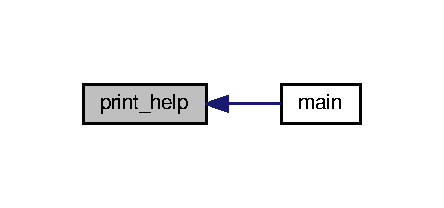
\includegraphics[width=213pt]{hello_8c_a6fc4beeab8ac72edc27edc24cf7ef525_icgraph}
\end{center}
\end{figure}


\index{hello.\+c@{hello.\+c}!print\+\_\+simbols@{print\+\_\+simbols}}
\index{print\+\_\+simbols@{print\+\_\+simbols}!hello.\+c@{hello.\+c}}
\subsubsection[{\texorpdfstring{print\+\_\+simbols(const char $\ast$)}{print_simbols(const char *)}}]{\setlength{\rightskip}{0pt plus 5cm}static void print\+\_\+simbols (
\begin{DoxyParamCaption}
\item[{const char $\ast$}]{greeting\+\_\+msg}
\end{DoxyParamCaption}
)\hspace{0.3cm}{\ttfamily [static]}}\hypertarget{hello_8c_a9327e4e5f8a3d809ecf0e564973b091b}{}\label{hello_8c_a9327e4e5f8a3d809ecf0e564973b091b}
Вывод строки в верхнем регистре Print greeting message and exit. 

Here is the caller graph for this function\+:\nopagebreak
\begin{figure}[H]
\begin{center}
\leavevmode
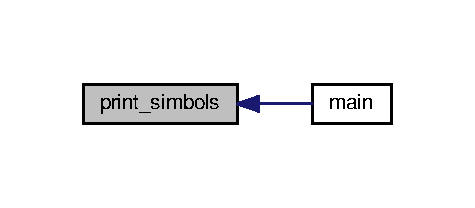
\includegraphics[width=228pt]{hello_8c_a9327e4e5f8a3d809ecf0e564973b091b_icgraph}
\end{center}
\end{figure}


\index{hello.\+c@{hello.\+c}!print\+\_\+version@{print\+\_\+version}}
\index{print\+\_\+version@{print\+\_\+version}!hello.\+c@{hello.\+c}}
\subsubsection[{\texorpdfstring{print\+\_\+version(void)}{print_version(void)}}]{\setlength{\rightskip}{0pt plus 5cm}static void print\+\_\+version (
\begin{DoxyParamCaption}
\item[{void}]{}
\end{DoxyParamCaption}
)\hspace{0.3cm}{\ttfamily [static]}}\hypertarget{hello_8c_a2e0d36c06cdd7fbacb264c67367d3b01}{}\label{hello_8c_a2e0d36c06cdd7fbacb264c67367d3b01}
Выводит информацию о справке

Print version and copyright information. xgettext\+: no-\/wrap

It is important to separate the year from the rest of the message, as done here, to avoid having to retranslate the message when a new year comes around. 

Here is the caller graph for this function\+:\nopagebreak
\begin{figure}[H]
\begin{center}
\leavevmode
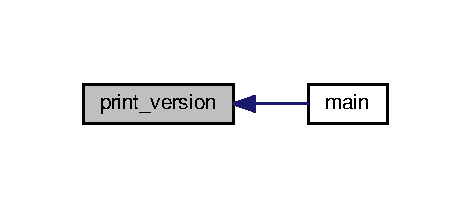
\includegraphics[width=226pt]{hello_8c_a2e0d36c06cdd7fbacb264c67367d3b01_icgraph}
\end{center}
\end{figure}




\subsection{Variable Documentation}
\index{hello.\+c@{hello.\+c}!longopts@{longopts}}
\index{longopts@{longopts}!hello.\+c@{hello.\+c}}
\subsubsection[{\texorpdfstring{longopts}{longopts}}]{\setlength{\rightskip}{0pt plus 5cm}const struct option longopts\mbox{[}$\,$\mbox{]}\hspace{0.3cm}{\ttfamily [static]}}\hypertarget{hello_8c_a7f2c8becae59a68faf6fc1540e88ab11}{}\label{hello_8c_a7f2c8becae59a68faf6fc1540e88ab11}
{\bfseries Initial value\+:}
\begin{DoxyCode}
= \{
  \{\textcolor{stringliteral}{"greeting"}, required\_argument, NULL, \textcolor{charliteral}{'g'}\},
  \{\textcolor{stringliteral}{"help"}, no\_argument, NULL, \textcolor{charliteral}{'h'}\},
  \{\textcolor{stringliteral}{"traditional"}, no\_argument, NULL, \textcolor{charliteral}{'t'}\},
  \{\textcolor{stringliteral}{"version"}, no\_argument, NULL, \textcolor{charliteral}{'v'}\},
  \{\textcolor{stringliteral}{"gtk"}, no\_argument, NULL, \textcolor{charliteral}{'w'}\},
  \{NULL, 0, NULL, 0\}
\}
\end{DoxyCode}
\hyperlink{hello_8c}{hello.\+c} -- print a greeting message and exit.

Copyright 1992-\/2017 Free Software Foundation, Inc.

This program is free software\+: you can redistribute it and/or modify it under the terms of the G\+NU General Public License as published by the Free Software Foundation, either version 3 of the License, or (at your option) any later version.

This program is distributed in the hope that it will be useful, but W\+I\+T\+H\+O\+UT A\+NY W\+A\+R\+R\+A\+N\+TY; without even the implied warranty of M\+E\+R\+C\+H\+A\+N\+T\+A\+B\+I\+L\+I\+TY or F\+I\+T\+N\+E\+SS F\+OR A P\+A\+R\+T\+I\+C\+U\+L\+AR P\+U\+R\+P\+O\+SE. See the G\+NU General Public License for more details.

You should have received a copy of the G\+NU General Public License along with this program. If not, see \href{https://www.gnu.org/licenses/}{\tt https\+://www.\+gnu.\+org/licenses/}.

Структура ключей и их символьных значений 
\hypertarget{system_8h}{}\section{src/system.h File Reference}
\label{system_8h}\index{src/system.\+h@{src/system.\+h}}
{\ttfamily \#include $<$limits.\+h$>$}\\*
{\ttfamily \#include $<$locale.\+h$>$}\\*
{\ttfamily \#include $<$stdio.\+h$>$}\\*
{\ttfamily \#include $<$stdlib.\+h$>$}\\*
{\ttfamily \#include $<$string.\+h$>$}\\*
{\ttfamily \#include $<$getopt.\+h$>$}\\*
{\ttfamily \#include $<$unistd.\+h$>$}\\*
{\ttfamily \#include $<$wchar.\+h$>$}\\*
{\ttfamily \#include $<$wctype.\+h$>$}\\*
{\ttfamily \#include \char`\"{}gettext.\+h\char`\"{}}\\*
{\ttfamily \#include \char`\"{}closeout.\+h\char`\"{}}\\*
Include dependency graph for system.\+h\+:\nopagebreak
\begin{figure}[H]
\begin{center}
\leavevmode
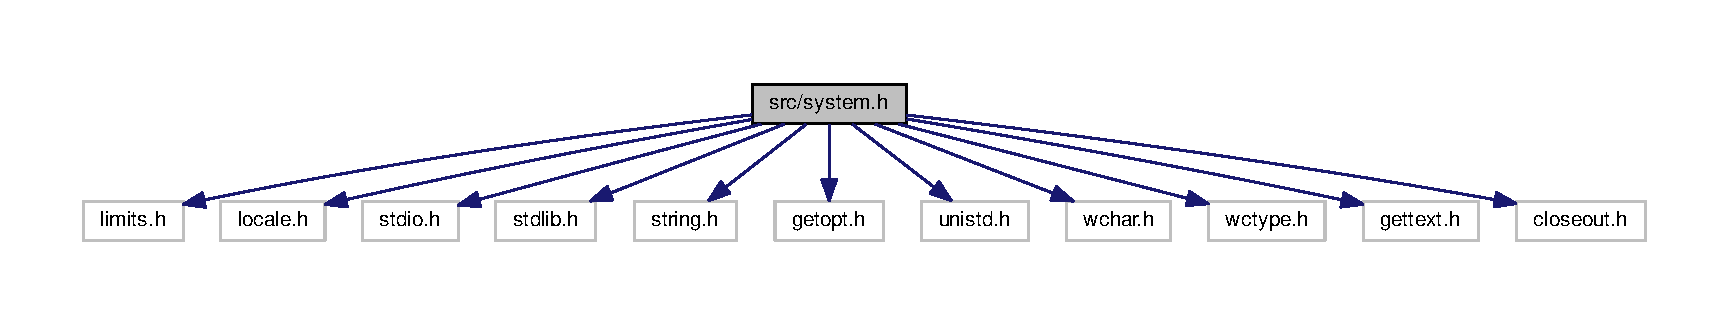
\includegraphics[width=350pt]{system_8h__incl}
\end{center}
\end{figure}
This graph shows which files directly or indirectly include this file\+:\nopagebreak
\begin{figure}[H]
\begin{center}
\leavevmode
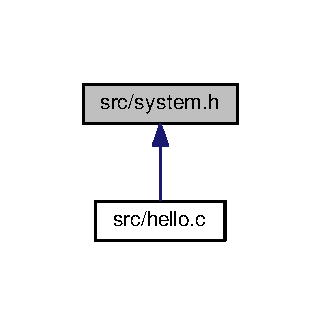
\includegraphics[width=154pt]{system_8h__dep__incl}
\end{center}
\end{figure}
\subsection*{Macros}
\begin{DoxyCompactItemize}
\item 
\#define \hyperlink{system_8h_a6554a5ea005e85d0f84f2f34c11de938}{\+\_\+}(str)~gettext (str)
\item 
\#define \hyperlink{system_8h_a2091f4107eaba5336ec06bb5e38a5711}{N\+\_\+}(str)~gettext\+\_\+noop (str)
\item 
\#define \hyperlink{system_8h_a88833a66d58e497c92d702140ac2883c}{S\+T\+R\+N\+C\+M\+P\+\_\+\+L\+IT}(s,  literal)~strncmp (s, \char`\"{}\char`\"{} literal \char`\"{}\char`\"{}, sizeof (literal) -\/ 1)
\end{DoxyCompactItemize}


\subsection{Macro Definition Documentation}
\index{system.\+h@{system.\+h}!\+\_\+@{\+\_\+}}
\index{\+\_\+@{\+\_\+}!system.\+h@{system.\+h}}
\subsubsection[{\texorpdfstring{\+\_\+}{_}}]{\setlength{\rightskip}{0pt plus 5cm}\#define \+\_\+(
\begin{DoxyParamCaption}
\item[{}]{str}
\end{DoxyParamCaption}
)~gettext (str)}\hypertarget{system_8h_a6554a5ea005e85d0f84f2f34c11de938}{}\label{system_8h_a6554a5ea005e85d0f84f2f34c11de938}
\index{system.\+h@{system.\+h}!N\+\_\+@{N\+\_\+}}
\index{N\+\_\+@{N\+\_\+}!system.\+h@{system.\+h}}
\subsubsection[{\texorpdfstring{N\+\_\+}{N_}}]{\setlength{\rightskip}{0pt plus 5cm}\#define N\+\_\+(
\begin{DoxyParamCaption}
\item[{}]{str}
\end{DoxyParamCaption}
)~gettext\+\_\+noop (str)}\hypertarget{system_8h_a2091f4107eaba5336ec06bb5e38a5711}{}\label{system_8h_a2091f4107eaba5336ec06bb5e38a5711}
\index{system.\+h@{system.\+h}!S\+T\+R\+N\+C\+M\+P\+\_\+\+L\+IT@{S\+T\+R\+N\+C\+M\+P\+\_\+\+L\+IT}}
\index{S\+T\+R\+N\+C\+M\+P\+\_\+\+L\+IT@{S\+T\+R\+N\+C\+M\+P\+\_\+\+L\+IT}!system.\+h@{system.\+h}}
\subsubsection[{\texorpdfstring{S\+T\+R\+N\+C\+M\+P\+\_\+\+L\+IT}{STRNCMP_LIT}}]{\setlength{\rightskip}{0pt plus 5cm}\#define S\+T\+R\+N\+C\+M\+P\+\_\+\+L\+IT(
\begin{DoxyParamCaption}
\item[{}]{s, }
\item[{}]{literal}
\end{DoxyParamCaption}
)~strncmp (s, \char`\"{}\char`\"{} literal \char`\"{}\char`\"{}, sizeof (literal) -\/ 1)}\hypertarget{system_8h_a88833a66d58e497c92d702140ac2883c}{}\label{system_8h_a88833a66d58e497c92d702140ac2883c}

%--- End generated contents ---

% Index
\backmatter
\newpage
\phantomsection
\clearemptydoublepage
\addcontentsline{toc}{chapter}{Index}
\printindex

\end{document}
